
% PDF
%\documentclass[pdftex,leqno,fleqn]{rapport}
%\documentclass[pdlaftex,leqno,fleqn]{article}

% DVI - PS
\documentclass[pdftex,leqno,fleqn,12pt]{article}

%%%%%%%%%%%%%%%%%%%%%%%%%%%%%%%%%%%%%%%%%%%%%%%%%%%%%%%%%%%%%%%%%%%%%%% PACKAGES

\usepackage[latin1]{inputenc}   % Ce qu'il faut pour document en fran\c{c}ais
%\usepackage[cyr]{aeguill}       % pour afficher � �
\usepackage{xspace}

%\usepackage{url}                % Pour afficher correctement les URLs
\usepackage{graphicx}           % Pour afficher les graphiques
\usepackage{subfigure}
\usepackage{latexsym}           % Plusieurs packages pour polices sp\'{e}ciales et math
\usepackage{amsmath}
\usepackage{amssymb}
\usepackage{amsfonts}

%\usepackage{algorithmic}
\usepackage{theorem}            % Pour les th\'{e}or\`{e}mes
%\usepackage{macros}

\usepackage{ulem}

\usepackage[sort&compress,numbers]{natbib}

\newcommand{\mnote}[1]{%
    \setlength{\marginparsep}{0.1in}
    \marginpar[\flushright\tiny\fbox{\parbox{0.5in}{\raggedright#1}}]
    {\flushleft\tiny\fbox{\parbox{0.5in}{\raggedright#1}}}}

\newcommand{\tabul}{\mbox{\ \ \ \ }}


\newtheorem{thm}{Theorem}[section]
\newtheorem{cor}[thm]{Corollary}
\newtheorem{lem}[thm]{Lemma}
\newtheorem{claim}[thm]{Claim}
\newtheorem{axiom}[thm]{Axiom}
\newtheorem{conj}[thm]{Conjecture}
\newtheorem{fact}[thm]{Fact}
\newtheorem{hypo}[thm]{Hypothesis}
\newtheorem{assum}[thm]{Assumption}
\newtheorem{prop}[thm]{Proposition}
\newtheorem{crit}[thm]{Criterion}
\newtheorem{defn}[thm]{Definition}
\newtheorem{notn}[thm]{Notation}
\newtheorem{exmp}[thm]{Example}
\newtheorem{rem}[thm]{Remarque}
\newtheorem{prob}[thm]{Problem}
\newtheorem{prin}[thm]{Principle}
\newtheorem{alg}{Algorithm}
\newenvironment{proof}{{\bf Proof:} \rm}{\hfill $\square$ \medskip\\}

\newcommand{\dem}{\noindent\textit{Proof :}}

\newcommand{\old}[1]{{}}


\newcommand{\nsout}{\mbox{\rm{\sout{n}}}}


\begin{document}

% paper title
%\title{ABC}
%\author{}
%\date{Carleton University\\ Dec 2006}

%\maketitle

%\begin{abstract}

%\end{abstract}

\newcommand{\UDG}{{\rm{UDG}}}
\newcommand{\paz}{G_\lambda^\theta}
%%%%%%%%%%%%%%%%%%%%%%%%%%%%%%%%%%%%%%%%%%%%%%%%%%%%%%%%%%%%%%%%%%%%%%%%%%%%%

%\section{Introduction}

\section{}
Given a simple polygon $P$ with $n$ vertices, $k$ of which are reflex, the depth of a point $q$
is defined to be the minimal area obtained by the intersection of $P$ with any half-plane having $q$ 
on its boundary.

%Given a simple polygon $P$, find a point $q$, such that each line through $q$ divides polygon
%$P$ into two polygons. The goal is to find a point that maximize the size of the smallest 
%sub-polygon.

\begin{thm}
There exists a polygon $P$ with $k$ reflex vertices, such that no point
has a depth greater than  $\frac{area(P)}{2(k+1)} + \epsilon$, 
for $k \ge 1$ and $\epsilon >0$.
%having the above property has size greater than $\frac{area(P)}{2(k+1)}$ for $k \ge 1$. 
%(for $k=1$ it is $\frac{area(P)}{k+3}$).
\end{thm}
%
\begin{proof}
Figure~\ref{fig:k4} shows an example of a polygon, which does not contain any point
of depth greater than $\frac{area(P)}{2(k+1)} + \epsilon$. 
Notice that a point can be located inside or outside a pocket. 
In the former case (inside a pocket), the depth of a point is bounded
by the area of the pocket, which is $\frac{area(P)}{2(k+1)}$.
In the later case, a point outside a pocket
has a depth smaller than $\frac{area(P)}{2(k+1)} + \epsilon$. 

\begin{figure}
   \begin{center}
    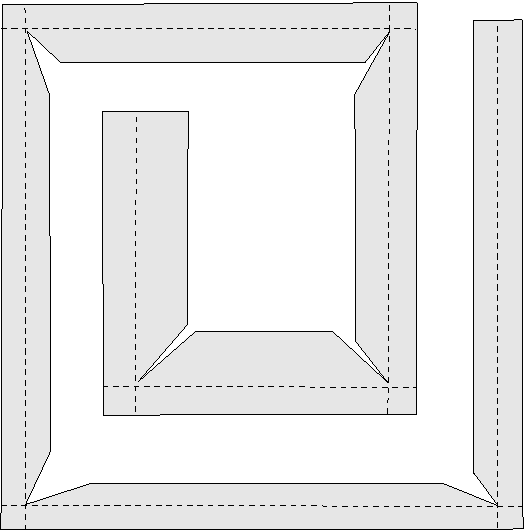
\includegraphics{OneOver2k.pdf}
   \end{center}
   \caption{Upper bound}
 \label{fig:k4}
\end{figure}

\end{proof}


%%%%%%%%%%%%%%%%%%%%%%%%%%%%%%%%%%%%%%%%%%%%%%%%%%
%%%%%%%%%%%%%%%%%%%  Lower bound  %%%%%%%%%%%%%%%%
%%%%%%%%%%%%%%%%%%%%%%%%%%%%%%%%%%%%%%%%%%%%%%%%%%
\begin{thm}
\label{thm:low}
For any simple polygon $P$ with $k \ge 1$ reflex vertices, there 
exists a point of depth greater than $\frac{area(P)}{2(k+1)}$.
\end{thm}
%
\begin{proof}
For simplicity, we prove the theorem on its discrete version.
In the discrete version, we are given a polygon $P$ and a set 
$N \subset P$ of points. The depth of a point $q$ is defined to be the 
minimal number of points in $N$ contained in the intersection 
of $P$ with any half-plane having $q$ on its boundary.

We first prove the theorem for the case where 
there is exactly one reflex vertex ($k=1$).

\begin{claim} 
\label{cl:oneRef}
For any polygon $P$ with one reflex vertex $r$ and a set $N \subset P$, 
there exists a point $q$ of depth greater or equal to $|N|/4$. 
\end{claim}
%
\begin{proof}

\begin{figure}
   \begin{center}
    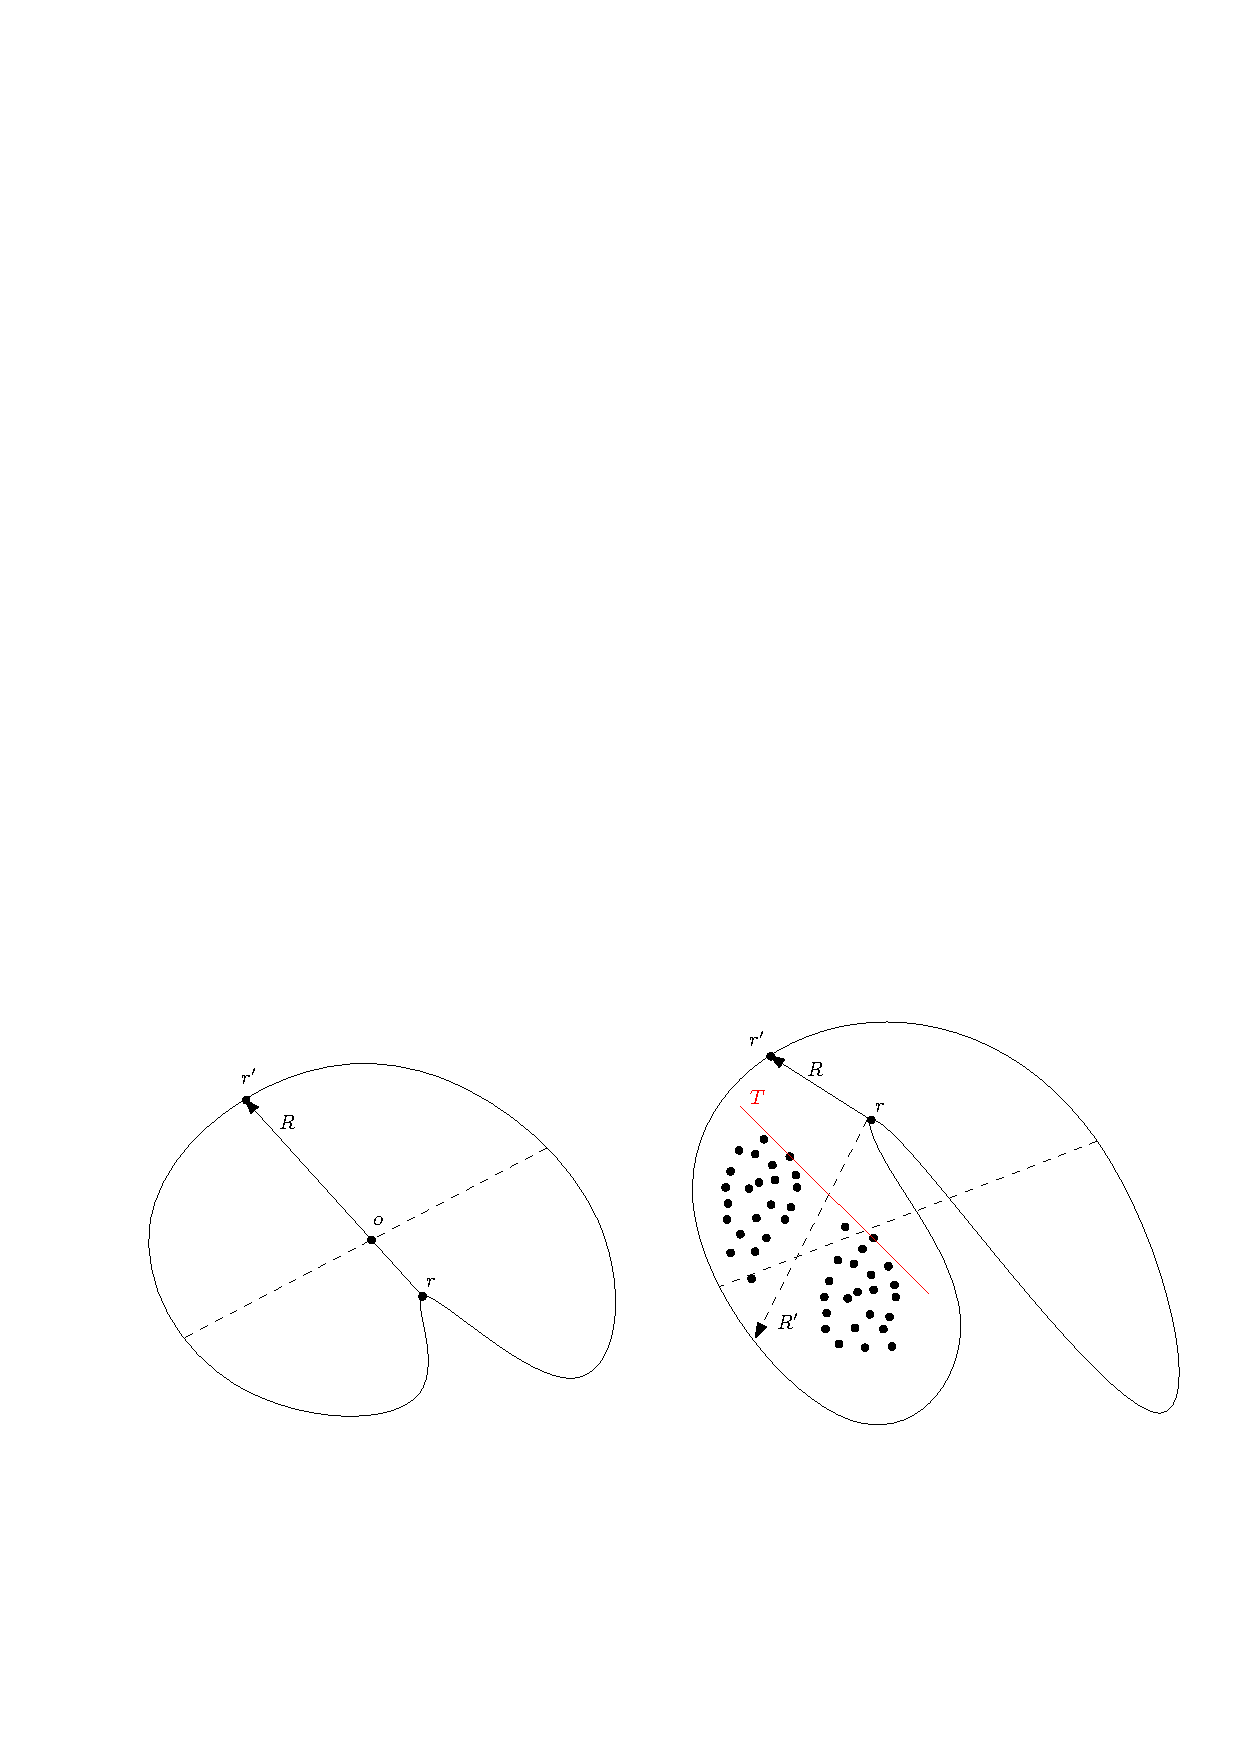
\includegraphics[scale=0.7]{oneReflex.pdf}
   \end{center}
   \caption{lower bound with one reflex vertex}
 \label{fig:tan}
\end{figure}

Draw a ray $R$ emanating from $r$ that divides $P$ 
into two sub-polygons $P_1$ and $P_2$, such that each sub-polygon contains $|N|/2$ points. 
Let $r'$ be the intersection point of $R$ and $P$.
According to Hum-Sandwich theorem, there is a line $l$ that splits both $P_1$ and $P_2$ into sub-polygons, each contains $|N|/4$ points.
Let $o$ be the intersection point of $l$ and $R$.

\begin{enumerate}
\item Point $o$ lies on the segment $\overline{rr'}$. \\
In this case, we choose $o$ to be the requested point. Notice that 
each half-plane that goes through $o$ contains at least $|N|/4$ points. 
Therefore, the depth of point $o$ is at least $|N|/4$. 

\item Point $o$ does not lay on the segment $\overline{rr'}$. \\
W.L.O.G let $P_1$ be a convex polygon (at least one of the two polygons $P_1$ and $P_2$ is convex.)
Draw a ray $R'$ emanating from $r$ that divides $P_1$ 
into two sub-polygons $P'_1$ and $P''_1$, each contains $|N|/4$ points.
For each set of points inside $P'_1$ and $P''_1$, compute the convex hull.
Let $T$ be the tangent of these two convex hulls, such that the half-plane having $T$ on its boundary and not containing $r$, contains all the points in $P_1$ (see Figure~\ref{fig:tan}).
Notice that the intersection point of $T$ and $R'$ has depth of at least $|N|/4$.
 
\end{enumerate} 

\end{proof}




Next, we prove the theorem for a polygon with $k>1$ reflex vertices.
\begin{claim} 
For any simple polygon $P$ with $k>1$ reflex vertices and a set $N \subset P$, 
there exists a point $q$ of depth greater or equal to $\frac{|N|}{2(k+1)}$.
\end{claim}
%
\begin{proof}

\begin{figure}
   \begin{center}
    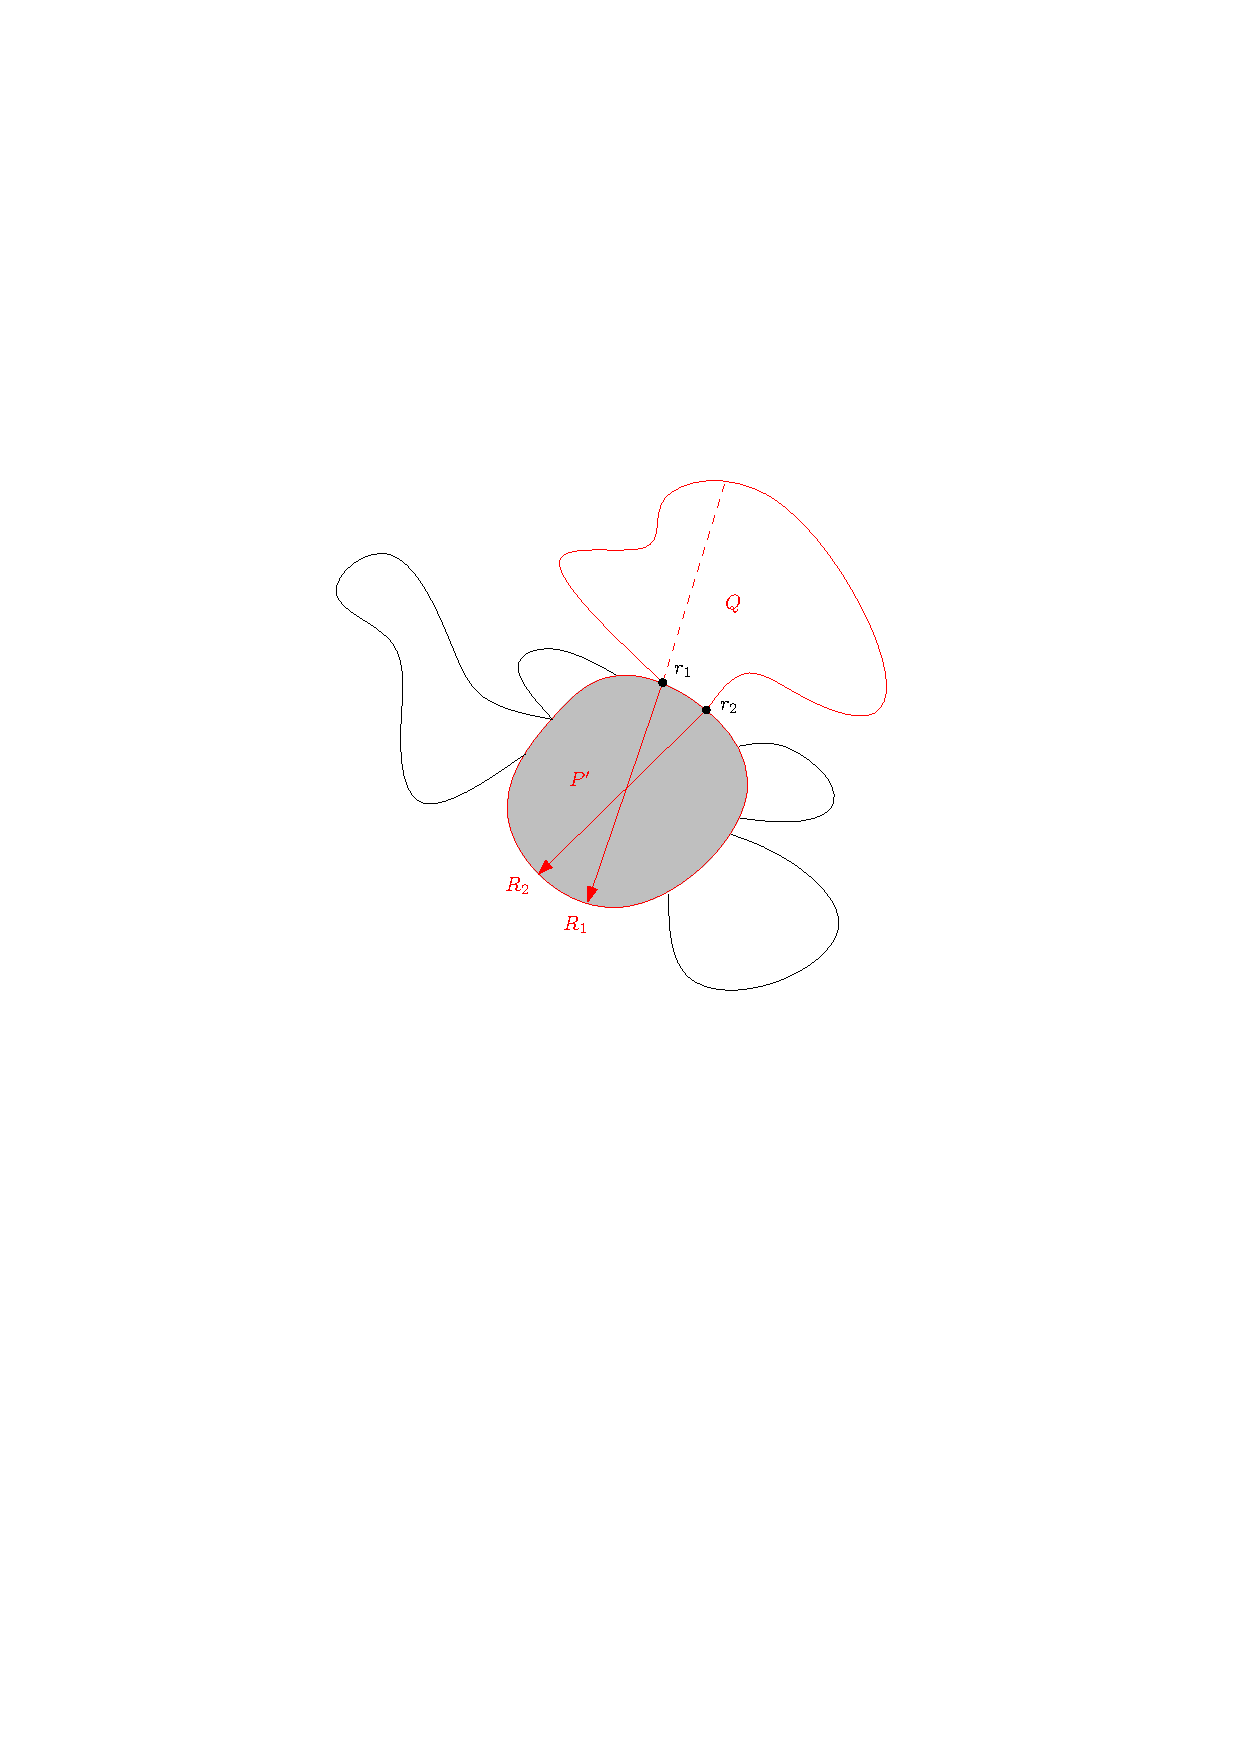
\includegraphics[scale=0.7]{Lowerbound1.pdf}
   \end{center}
   \caption{Lower bound}
 \label{fig:LB1}
\end{figure}

Divide polygon $P$ into at most $k+1$ convex sub-polygons.
Let $P'$ be a convex sub-polygon that contains the most points. 
Clearly, polygon $P'$ contains more than $\frac{|N|}{(k+1)}$ points. 
Let $Q$ be the largest simple polygon within $P$ that contains the maximal number of points (of $N$),
and intersects $P'$ only on its boundary. 
Let $r_1$ and $r_2$ be the two intersection points of $P'$ and $Q$. 
Draw a ray $R_1$ emanating from $r_1$ that divides $P'$ 
into two sub-polygons $P'_1$ and $P''_1$, each contains $\frac{|N|}{2(k+1)}$ points. 
Similarly, draw a ray $R_2$ emanating from $r_2$ that divides $P'$ 
into two sub-polygons $P'_2$ and $P''_2$, each contains at least $\frac{|N|}{2(k+1)}$ points.
If $Q$ contains less points than $\frac{|N|}{(k+1)}$, then we decrease $P'$, until $Q$ contains  $\frac{|N|}{(k+1)}$ points.

Extend $R_1$ (alternatively $R_2$) in the other direction until it intersects $P$.
This extension divides polygon $Q$ into two sub-polygons $Q_1$ and $Q'_1$ (alternatively $Q_2$ and $Q'_2$).
If the sub-polygon $Q_1$ that does not contain $r_2$ (alternatively $Q_2$ that does not contain $r_1$) 
has more than  $\frac{|N|}{2(k+1)}$ points, then we are done (this is like in Claim~\ref{cl:oneRef} case 2).

Otherwise, we start sweeping from $r_1$ along the edge $(r_1,r_2)$ 
while maintaining that the ray (of the sweep) divides $P'$ into two sub-polygons, 
with the same number of points. 
Notice that we start with sub-polygon $Q_1^*=Q_1$ ($Q_1^*$ represents the expending of $Q_1$ during the sweep)
that has less than $\frac{|N|}{2(k+1)}$ points, and in the end of the sweep 
$Q_1^*$  ($Q_1^*$ contains $r_2$)
%(we denote $Q_1^*$ as $Q_1$ during the sweep) 
contains at least $\frac{|N|}{2(k+1)}$ points. 
%Recall that the sub-polygon of $Q_2$ obtained by the 
%extension of ray $R_2$ in the other direction, that does not contain $r_1$, 
%has less than $\frac{|N|}{2(k+1)}$ points.
Therefore, there is a (balanced) point along the edge $(r_1,r_2)$ in the sweep,
where $Q_1^*$ change the number of points 
it contains from less than $\frac{|N|}{2(k+1)}$ points to at least $\frac{|N|}{2(k+1)}$ points.
The depth of this (balanced) point is at least $\frac{|N|}{2(k+1)}$ 
%
%and there is a point along the edge $(r_1,r_2)$,
%where this sub-polygon (which by now is extended) has at least $\frac{|N|}{2(k+1)}$ points.
%Recall that the sub-polygon of $Q$ obtained by the extension ray $R_2$ in the other direction,
%that does not contain $r_1$, has less than $\frac{|N|}{2(k+1)}$ points.
%Hence, the sub-polygon of $Q$ obtained by the extension ray $R_2$ in the other direction,
%that contains $r_1$, has more or equal to $\frac{|N|}{2(k+1)}$ points.
%Therefore, There must be such a portal (balanced) point along the sweeping, 
%and this point has depth greater or equal to $\frac{|N|}{2(k+1)}$ 
%
(this is similar to Claim~\ref{cl:oneRef} case 1). 

\end{proof}

\end{proof}








\end{document}
